\documentclass[a4paper,11pt]{book}
%\documentclass[a4paper,twoside,11pt,titlepage]{book}
\usepackage{listings}
\usepackage[utf8]{inputenc}
\usepackage[spanish]{babel}
% Para las formulas
\usepackage{amsmath}
\usepackage{amssymb}
% Para la bibliografia
\usepackage[square,numbers]{natbib}
% Para que separe bien los parrafos
%\renewcommand{\baselinestretch}{1.25}
%\setlength{\parskip}{1mm}
% Para la visualizacion del simbolo del euro en la parte de gastos
\usepackage{eurosym}

% \usepackage[style=list, number=none]{glossary} %
%\usepackage{titlesec}
%\usepackage{pailatino}

\decimalpoint
\usepackage{dcolumn}
\newcolumntype{.}{D{.}{\esperiod}{-1}}
\makeatletter
\addto\shorthandsspanish{\let\esperiod\es@period@code}
\makeatother


\usepackage[chapter]{algorithm}
\RequirePackage{verbatim}
%\RequirePackage[Glenn]{fncychap}
\usepackage{fancyhdr}
\usepackage{graphicx}
\usepackage{afterpage}

\usepackage{longtable}

\usepackage[pdfborder={000}]{hyperref} %referencia

% ********************************************************************
% Re-usable information
% ********************************************************************
\newcommand{\myTitle}{Implementación en tiempo real de sistemas de identificación de tráfico de red}
\newcommand{\myDegree}{Grado en Ingeniería Informática}
\newcommand{\myName}{Álvaro Maximino Linares Herrera}
\newcommand{\myProf}{Jesús Esteban Díaz Verdejo}
\newcommand{\myOtherProf}{Nombre Apllido1 Apellido2 (tutor2)\xspace}
%\newcommand{\mySupervisor}{Put name here\xspace}
\newcommand{\myFaculty}{Escuela Técnica Superior de Ingenierías Informática y de Telecomunicación\xspace}
\newcommand{\myFacultyShort}{E.T.S. de Ingenierías Informática y de
Telecomunicación\xspace}
\newcommand{\myDepartment}{Departamento de ...\xspace}
\newcommand{\myUni}{\protect{Universidad de Granada}\xspace}
\newcommand{\myLocation}{Granada\xspace}
\newcommand{\myTime}{\today\xspace}
\newcommand{\myVersion}{Version 0.1\xspace}


\hypersetup{
pdfauthor = {\myName (email (en) ugr (punto) es)},
pdftitle = {\myTitle},
pdfsubject = {},
pdfkeywords = {palabra_clave1, palabra_clave2, palabra_clave3, ...},
pdfcreator = {LaTeX con el paquete ....},
pdfproducer = {pdflatex}
}

%\hyphenation{}


%\usepackage{doxygen/doxygen}
%\usepackage{pdfpages}
\usepackage{url}
\usepackage{colortbl,longtable}
\usepackage[stable]{footmisc}
%\usepackage{index}

%\makeindex
%\usepackage[style=long, cols=2,border=plain,toc=true,number=none]{glossary}
% \makeglossary

% Definición de comandos que me son tiles:
%\renewcommand{\indexname}{Índice alfabético}
%\renewcommand{\glossaryname}{Glosario}

\pagestyle{fancy}
\fancyhf{}
\fancyhead[LO]{\leftmark}
\fancyhead[RE]{\rightmark}
\fancyhead[RO,LE]{\textbf{\thepage}}
\renewcommand{\chaptermark}[1]{\markboth{\textbf{#1}}{}}
\renewcommand{\sectionmark}[1]{\markright{\textbf{\thesection. #1}}}
%Para subsubsection
\setcounter{tocdepth}{3}% Include \subsubsection in ToC
\setcounter{secnumdepth}{3}% Number \subsubsection
%Para las ecuaciones
\renewcommand{\theequation}{\arabic{equation}}
\newcounter{neq}

\newcommand{\intro}{\\ \smallskip}

\setlength{\headheight}{1.5\headheight}

\newcommand{\HRule}{\rule{\linewidth}{0.5mm}}
%Definimos los tipos teorema, ejemplo y definición podremos usar estos tipos
%simplemente poniendo \begin{teorema} \end{teorema} ...
\newtheorem{teorema}{Teorema}[chapter]
\newtheorem{ejemplo}{Ejemplo}[chapter]
\newtheorem{definicion}{Definición}[chapter]

\definecolor{gray97}{gray}{.97}
\definecolor{gray75}{gray}{.75}
\definecolor{gray45}{gray}{.45}
\definecolor{gray30}{gray}{.94}

\lstset{ frame=Ltb,
     framerule=0.5pt,
     aboveskip=0.5cm,
     framextopmargin=3pt,
     framexbottommargin=3pt,
     framexleftmargin=0.1cm,
     framesep=0pt,
     rulesep=.4pt,
     backgroundcolor=\color{gray97},
     rulesepcolor=\color{black},
     %
     stringstyle=\ttfamily,
     showstringspaces = false,
     basicstyle=\scriptsize\ttfamily,
     commentstyle=\color{gray45},
     keywordstyle=\bfseries,
     %
     numbers=left,
     numbersep=6pt,
     numberstyle=\tiny,
     numberfirstline = false,
     breaklines=true,
   }
 
% minimizar fragmentado de listados
\lstnewenvironment{listing}[1][]
   {\lstset{#1}\pagebreak[0]}{\pagebreak[0]}

\lstdefinestyle{CodigoC}
   {
	basicstyle=\scriptsize,
	frame=single,
	language=C,
	numbers=left
   }
\lstdefinestyle{CodigoC++}
   {
	basicstyle=\small,
	frame=single,
	backgroundcolor=\color{gray30},
	language=C++,
	numbers=left
   }

 
\lstdefinestyle{Consola}
   {basicstyle=\scriptsize\bf\ttfamily,
    backgroundcolor=\color{gray30},
    frame=single,
    numbers=none
   }


\newcommand{\bigrule}{\titlerule[0.5mm]}


%Para conseguir que en las páginas en blanco no ponga cabecerass
\makeatletter
\def\clearpage{%
  \ifvmode
    \ifnum \@dbltopnum =\m@ne
      \ifdim \pagetotal <\topskip
        \hbox{}
      \fi
    \fi
  \fi
  \newpage
  \thispagestyle{empty}
  \write\m@ne{}
  \vbox{}
  \penalty -\@Mi
}
\makeatother

\usepackage{pdfpages}
\begin{document}
\begin{titlepage}
 
 
\newlength{\centeroffset}
\setlength{\centeroffset}{-0.5\oddsidemargin}
\addtolength{\centeroffset}{0.5\evensidemargin}
\thispagestyle{empty}

\noindent\hspace*{\centeroffset}\begin{minipage}{\textwidth}

\centering

\includegraphics[width=0.9\textwidth]{imagenes/logo_ugr.jpg}\\[1.4cm]

\textsc{ \Large TRABAJO FIN DE GRADO\\[0.2cm]}
\textsc{ INGENIERÍA EN INFORMÁTICA}\\[1cm]
% Upper part of the page
% 
% Title
{\Huge\bfseries \myTitle\\
}
\noindent\rule[-1ex]{\textwidth}{3pt}\\[3.5ex]
{\large\bfseries} %Cambio aqui
\end{minipage}

\vspace{2.5cm}
\noindent\hspace*{\centeroffset}\begin{minipage}{\textwidth}
\centering

\textbf{Autor}\\ {\myName}\\[2.5ex]
\textbf{Directores}\\
{\myProf}\\[2cm]

\includegraphics[width=0.3\textwidth]{imagenes/etsiit_logo.png}\\[0.1cm]
\textsc{Escuela Técnica Superior de Ingenierías Informática y de Telecomunicación}\\
\textsc{---}\\
Granada, 11 de septiembre de 2017
\end{minipage}
%\addtolength{\textwidth}{\centeroffset}
%\vspace{\stretch{2}}
\end{titlepage}



\chapter*{}
%\thispagestyle{empty}
%\cleardoublepage

%\thispagestyle{empty}

\begin{titlepage}
 
 
\setlength{\centeroffset}{-0.5\oddsidemargin}
\addtolength{\centeroffset}{0.5\evensidemargin}
\thispagestyle{empty}

\noindent\hspace*{\centeroffset}\begin{minipage}{\textwidth}

\centering
%
\includegraphics[width=0.9\textwidth]{imagenes/logo_ugr.jpg}\\[1.4cm]

%\textsc{ \Large PROYECTO FIN DE CARRERA\\[0.2cm]}
%\textsc{ INGENIERÍA EN INFORMÁTICA}\\[1cm]
% Upper part of the page
% 

 \vspace{3.3cm}

%si el proyecto tiene logo poner aquí

\includegraphics{imagenes/logo.png} 
 \vspace{0.5cm}

% Title

{\Huge\bfseries \myTitle\\
}
\noindent\rule[-1ex]{\textwidth}{3pt}\\[3.5ex]
{\large\bfseries Subtitulo del proyecto\\[4cm]} %Cambio aqui
\end{minipage}

\vspace{2.5cm}
\noindent\hspace*{\centeroffset}\begin{minipage}{\textwidth}
\centering

\textbf{Autor}\\ {\myName}\\[2.5ex]
\textbf{Directores}\\
{\myProf}\\[2cm]
%
\includegraphics[width=0.15\textwidth]{imagenes/tstc.png}\\[0.1cm]
%\textsc{Departamento de Teoría de la Señal, Telemática y Comunicaciones}\\
%\textsc{---}\\
%Granada, mes de 201
\end{minipage}
%\addtolength{\textwidth}{\centeroffset}
\vspace{\stretch{2}}

 
\end{titlepage}






\cleardoublepage
\thispagestyle{empty}

\begin{center}
{\large\bfseries \myTitle}\\
\end{center}
\begin{center}
%{\myName}\\
\myName\\
\end{center}

%\vspace{0.7cm}
\noindent{\textbf{Palabras clave}: identificación de tráfico, Monitor de Red, clasificación de tráfico, calidad de servicio, Bro}\\

\vspace{0.7cm}
\noindent{\textbf{Resumen}}\\
La identificación de tráfico consiste en asignar instancias de tráfico al tipo de aplicaciones que generaron dicho tráfico, esto sirve para realizar una clasificación del mismo, permitiendo así encontrar fallos en cuanto a la calidad de servicio, fallos en el sistema o detectar ataques.
\intro Las técnicas hasta ahora usadas o han quedado obsoletas, cómo por ejemplo la identificación mediante puertos, o no tienen buen rendimiento, cómo las basadas en aprendizaje automático, o no respetan la privacidad, cómo la Inspección Profunda de Paquetes. Por lo tanto, es necesario la utilización de una nueva técnica que permita una identificación precisa, rápida y que respete la privacidad.
\intro En el presente trabajo se abordará la creación de un módulo para un Monitor de Redes, en el que se implemente la técnica propuesta por los investigadores del departamento de Teoría de la Señal, Telemática y Comunicaciones de la Universidad de Granada. Dicha técnica permite resolver los problemas anteriores, obteniendo además una tasa de identificación correcta más alta que en las otras técnicas.
\intro Se probará que dicho módulo funciona de forma correcta mediante el uso de trazas de tráfico de prueba, llevándola después a escenarios reales.
\cleardoublepage


\thispagestyle{empty}


\begin{center}
{\large\bfseries Implementation on real time of traffic network identification systems}\\
\end{center}
\begin{center}
Álvaro Maximino Linares Herrera\\
\end{center}

%\vspace{0.7cm}
\noindent{\textbf{Keywords}: traffic identification, Network Monitoring System, traffic classification, quality of service, Bro}\\

\vspace{0.7cm}
\noindent{\textbf{Abstract}}\\

The identification of traffic consists on assigning instances of traffic to the type of applications that generated that traffic. This 
is used to create a classification of what has been mentioned above, allowing to find mistakes regarding the quality of service, 
system failure or attacks detection.

\intro The techniques used until now has been either obsolete, such us the port-based identification, or do not have good performance, 
as the ones based on automatic learning or do not respect the privacy as Deep Package Inspection. Hence why is compulsory the use of a 
new technique which will allow a fast, accurate identification that will respect the privacy.

\intro In the following document, the creation of a module will be addressed for a network monitor, in which will be implemented the 
technique proposed by the researchers of the Theory of Signals, Telematics and Comunications of the University of Granada that would 
allow us to solve the above problems as well us providing us with a higher right identification rate than the other methods.

\intro The working status of this module will be tested with the use of traffic test traces, carried afterwards to real based 
scenarios.

\chapter*{}
\thispagestyle{empty}

\noindent\rule[-1ex]{\textwidth}{2pt}\\[4.5ex]

Yo, \textbf{\myName}, alumno de la titulación TITULACIÓN de la \textbf{Escuela Técnica Superior
de Ingenierías Informática y de Telecomunicación de la Universidad de Granada}, con DNI 76669401M, autorizo la
ubicación de la siguiente copia de mi Trabajo Fin de Grado en la biblioteca del centro para que pueda ser
consultada por las personas que lo deseen.

\vspace{6cm}

\noindent Fdo: \myName

\vspace{2cm}

\begin{flushright}
Granada a 11 de septiembre de 2017.
\end{flushright}


\chapter*{}
\thispagestyle{empty}

\noindent\rule[-1ex]{\textwidth}{2pt}\\[4.5ex]

D. \textbf{\myProf}, Profesor del Departamento Teoría de la Señal, Telemática y Comunicaciones (TSTC) de la Universidad de Granada.

\vspace{0.5cm}

%D. \textbf{Nombre Apellido1 Apellido2 (tutor2)}, Profesor del Área de XXXX del Departamento YYYY de la Universidad de Granada.


%\vspace{0.5cm}

\textbf{Informa:}

\vspace{0.5cm}

Que el presente trabajo, titulado \textit{\textbf{\myTitle}},
ha sido realizado bajo su supervisión por \textbf{\myName}, y autorizamos la defensa de dicho trabajo ante el tribunal
que corresponda.

\vspace{0.5cm}

Y para que conste, expiden y firman el presente informe en Granada a 11 de septiembre de 2017.

\vspace{1cm}

\textbf{Los directores:}

\vspace{5cm}

\noindent \textbf{\myProf}

\chapter*{Agradecimientos}
\thispagestyle{empty}

       \vspace{1cm}

En primer lugar, dar las gracias a mi maravillosa familia, tanto a los que están, cómo a los que se han ido a lo largo de los años, por su confianza y cariño.
\intro También dar las gracias a Jesús, por su dedicación e inspiración, así como su paciencia con un alumno como yo.
\intro Por último, dar las gracias a mis amigos, por su apoyo incondicional. Y en especial a Carmen y a Javi.

%\frontmatter
\tableofcontents
%\listoffigures
%\listoftables
%
%\mainmatter
%\setlength{\parskip}{5pt}

\chapter{Introducción}

La clasificación de tráfico en red es una tarea importante 
en lo relativo a las comunicaciones, en un mundo cada vez 
más digitalizado e intercomunicado, lo que más importa es 
la seguridad y para ello es esencial la clasificación del 
tráfico, permitiendo detectar de forma temprana intrusiones 
y comportamientos anormales, para los cuales podremos 
prepararnos, de esta forma, por ejemplo, el encargado de un 
servidor podrá mantener la calidad de servicio, pues mediante 
ISP (Internet Service Provider) se puede establecer diferentes 
niveles de prioridad en el tráfico de red.
\intro
En este trabajo haremos uso de BRO, un NMS (Network Monitoring System), 
al cual mediante la implementación de técnicas de emparejamiento de 
flujos, lo dotaremos de la capacidad analítica de discernir que flujos 
son emparejables, y por lo tanto pertenecen a lo mismo.

\section{Conceptos básicos}

En este apartado vamos a aclarar los conceptos básicos que son necesarios 
para entender este trabajo.
\intro
Lo primero que tenemos que tener claro es lo que es un paquete. Un paquete 
es cada un fragmento de la información que queremos enviar a través de una red. 
Este paquete contiene datos sobre quiénes somos, digitalmente, y hacia donde 
enviamos la información, así que incluso un sólo paquete da mucha información 
sobre quienes somos en la red.
\intro
Lo siguiente que debemos de saber es que es un flujo, para ello tenemos que 
volver hacia la definición anterior, pues consiste en la historia de un grupo 
de paquetes, esto quiere decir cómo se mueven los paquetes a través de las capas 
de red, de datos y la física. Para quien no sepa sobre redes se estará 
preguntando que son estas capas, pues bien, estas capas son del modelo OSI, que 
es el modelo de referencia para los protocolos de red, siendo las distintas 
capas las siguientes:
\intro
1. Aplicación
2. Presentación
3. Sesión
4. Transporte
5. Red
6. Enlace de datos
7. Física
\intro
Lo siguiente que explicaremos será que es un NMS o Network Monitoring System, 
como el nombre nos indica consiste en un programa que se dedica a monitorizar 
el tráfico del sistema y en caso de encontrar algún problema avisará al 
administrador del sistema. En nuestro caso el NMS que usaremos será Bro, 
aunque existen otros.

\section{TCP y UDP}

Describir que es TCP y que UDP, poner imágenes del libro sobre la comunicación.
%
\chapter{Estado del arte}

Aquí se encuentra la parte teórica y tecnológica del proyecto. Se hablará de la identificación de tráfico y de 
las distintas técnicas que existen para ello. También se hablará de Bro \cite{broindex}, el 
analizador de tráfico que se usará para 
llevar a cabo el desarrollo del módulo. Se introducirá en que consiste, cómo gestiona los eventos y sus 
funcionalidades básicas, así como la posibilidad de ampliar estas.

\intro Por último se presentará de forma teórica en que consiste el emparejamiento de flujos y de qué forma 
se podría usar para identificar el tráfico.

\section{Identificación de tráfico}

Hay que tener claro que identificar el tráfico no es clasificarlo. Identificar el tráfico consiste en analizarlo 
y obtener patrones comunes con los cuales se pueda ordenar el tráfico de forma posterior. Algunas de los patrones 
que se pueden tener en cuenta a la hora de identificar tráfico son los puertos, las IP's o la clase a la que 
pertenece.

\intro Por lo tanto la identificación del tráfico de la red es esencial para realizar una clasificación 
posterior, la cual se podrá analizar en busca de amenazas o intrusos, a nivel de seguridad y componentes lentos 
o defectuosos que afecten al rendimiento del servicio. Para poder identificar el tráfico lo deseable es un 
método que sea rápido y proteja la privacidad de los distintos usuarios.

\subsection{Técnicas de identificación de tráfico}

Existen varias técnicas de identificación de tráfico, como ya se explicó anteriormente. Estas técnicas son 
el paso previo a la clasificación del tráfico. Podría considerarse que son el paso intermedio a la clasificación. 
El tráfico, hasta ahora, se puede identificar de la siguiente forma.

\begin{itemize}
\item Por los puertos de la capa de transporte, establecido por \textit{IANA}. \cite{iana}
\item Por el contenido del paquete o \textit{DPI}. \cite{payload}
\item Por la aplicación de técnicas de aprendizaje automático sobre estadísticas de tráfico, \textit{machine 
learning}. \cite{learning}
\end{itemize}

\intro En los siguientes apartados se verán estas técnicas de una forma más detallada.

\subsection{Identificación de tráfico basada en flujos}

Dentro de este ámbito se encuentran dos de las tres técnicas que se han presentado anteriormente.
\begin{itemize}

\item Identificación basada en los puertos de la capa de transporte. \cite{iana}

\intro Esta técnica consiste en identificar el tráfico dependiendo de los puertos de la capa de transporte, 
fue diseñada por IANA \cite{ianaexplicacion}. Esto se debe a que IANA es la organización que se encarga de 
asignar los protocolos de Internet, algunos nombres de dominios y coordinar la asignación de direcciones IP. 

\intro Por lo tanto, IANA es quien asigna el número de puerto a los distintos protocolos, haciendo que se pueda 
identificar el tráfico por el número de puerto al que se envía. Este sistema tiene el inconveniente de que 
ahora mismo, se están desarrollando multitud de aplicaciones web. Estas aplicaciones se conectan mediante el 
puerto 80, es decir, mediante el protocolo HTTP. Pero esto es en teoría , pues se puede hacer que cualquier 
aplicación envíe información por el puerto 80, sin que sea HTTP, lo cual daría como resultado una mala 
identificación y posterior clasificación.

\item Identificación basada en la aplicación de técnicas de aprendizaje automático sobre estadísticas 
de tráfico \cite{learning}.

\intro Esta clasificación es muy sencilla. Consta de algoritmos de aprendizaje automático, los cuales se 
dedican a realizar análisis estadísticos. De esta forma aprenden las características determinadas de 
los flujos. La clasificación de tráfico que se realiza con este método tiene un porcentaje de acierto 
del 95\%, según se puede leer en el artículo \cite{comparacion}.
\end{itemize}

\subsection{DPI}

\begin{itemize}

\item Identificación basada en el contenido del paquete o DPI. \cite{payload}

\intro Esta técnica de identificación consiste en analizar los paquetes, más allá de su cabecera. 
La Inspección Profunda de Paquetes, DPI por sus siglas en inglés, \textit{Deep Packet Inspection}. 
Esta técnica lo que hace es analizar todos los paquetes en busca de cadenas que se repitan, además 
de las IP's y los puertos. Una vez que tiene una cadena, la usa para buscar paquetes que tienen ese patrón, 
de esta forma establece un patrón de identificación.

\intro Esta técnica es útil para buscar virus, intrusiones y demás. Suele ser usada por los proveedores de 
servicios de Internet, ISP, \textit{Internet Service Provider} y grandes empresas. 
Se puede decir que es una técnica que no respeta la privacidad, pues entra dentro de la información del paquete, 
más allá de la cabecera. Aunque en el caso de una gran empresa si puede hacerse, pues si se está en la red propia 
no es delito mirar la información que contienen los paquetes. 

\intro En algunos países, como Alemania, donde es ilegal el uso de \textit{torrents}, 
las autoridades pueden pedir información al proveedor de servicios sobre uno de sus clientes, si cree que este 
está infringiendo la red, por lo que esta técnica es ideal para este tipo de cometidos.

\intro Además de para lo descrito, esta técnica también es ideal para saber si se está 
siendo atacado. \cite{dpiaproximacion}
\end{itemize}

\section{BRO}

Bro \cite{broindex}, es un analizador de tráfico de red de código abierto. Al ser de código abierto permite 
ser usado por quien lo desee sin necesidad de pagar licencias. Funciona sobre sistemas basados en Linux y 
Mac OS X. Una de sus principales características es la gran cantidad de información que devuelve con un solo 
escaneo. Otros monitores de red devuelven menos información, teniendo que ser el propio administrador el que 
analice después la información obtenida por estos. Por lo tanto tardará más en resolver los posibles problemas 
que encuentre en la red.

\begin{figure}[H]
  
\includegraphics[width=0.5\textwidth]{imagenes/logo-bro.png}
  \centering
  \caption{Logo de Bro.}
\end{figure}

\intro No tiene interfaz gráfica, por lo que su gestión se realiza desde la linea de comandos. Cuando se analiza 
tráfico, Bro generará unos registros, los cuales están divididos en función de parámetros definidos por parte del 
equipo que lo ha desarrollado.

\intro Bro incorpora la posibilidad de introducir funcionalidades nuevas, mediante la programación en su 
propio lenguaje de \textit{scripting}, del mismo nombre. Esto se desarrollará más adelante y en la 
parte de implementación se podrá ver cómo se desarrolla y algunos ejemplos de código escrito en Bro.

\intro El lenguaje de scripting está orientado a trabajar con eventos. Por lo tanto a la hora de añadir una nueva funcionalidad habrá que crearla a partir del uso de los eventos que puede gestionar Bro.

\intro \noindent Bro está estructurado de forma que todos los flujos de paquetes que analiza son procesados por el motor de eventos. Este motor convierte los flujos de paquetes en eventos, de forma que es más sencillo trabajar con ellos. 
Una vez que los eventos son procesados se generan los registros correspondientes, los cuales podrán ser analizados posteriormente. \cite{broarquitectura}

\begin{figure}[H]
  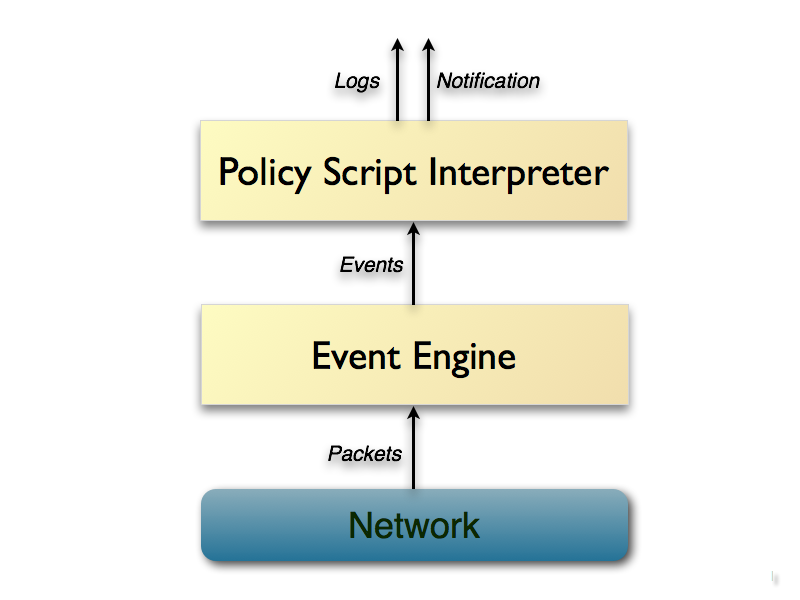
\includegraphics[width=0.5\textwidth]{imagenes/arquitectura-bro.png}
  \centering
  \caption{Arquitectura de Bro.}
\end{figure}

\subsection{Funcionalidades básicas de BRO}

La funcionalidad básica de Bro es la monitorización de la red en la que se ejecuta. 
Mientras que se encuentra en ejecución, genera registros o \textit{logs} en texto plano que se 
podrán leer usando un editor de texto. Si se analiza un archivo \textit{pcap} los logs no cambiarán. Sin 
embargo si se analiza tráfico a tiempo real, los registros se irán actualizando a medida que pase el tiempo. 
Algunos de los \textit{logs} que se generarán son los siguientes.

\begin{itemize}
\item \textit{dpd.log}. Consiste en un resumen de los protocolos encontrados en puertos que no son estándar.
\item \textit{dns.log}. Contendrá toda la actividad correspondiente al \textit{DNS}
\item \textit{ftp.log}. Un registro de la actividad a nivel de sesión de \textit{FTP}.
\item \textit{files.log}. Un resumen con los archivos transferidos a través de una red. Incluye 
protocolos \textit{HTTP, FTP y SMTP.}
\item \textit{http.log}. Registro de toda la actividad \textit{HTTP} con sus réplicas.
\item \textit{ssl.log}. Un registro de las sesiones \textit{SSL}, incluidos los certificados que se utilizan.
\item \textit{weird.log}. En este \textit{log} se guarda la información correspondiente a actividad 
inesperada o rara a nivel de protocolo. Al analizar gran cantidad de tráfico no es muy útil, pues ocurren 
muchas cosas raras, pero a pequeña escala es bastante interesante para detectar intrusiones y demás.
\item \textit{conn.log}. Aquí se puede ver la información correspondiente a conexiones  \textit{TCP, UDP e ICMP}.
\end{itemize}

\intro Para más información sobre \textit{logs} generados por una monitorización de Bro lea \cite{brologs}.

\intro Ahora con toda esta información, el administrador del sistema podrá determinar si existen amenazas en 
la red o si hay algún componente defectuoso.

\subsection{Eventos y trazas}

La programación en Bro no es secuencial, no se escribe un \textit{script} y se espera que se ejecute en el orden 
en el que está escrito. La programación aquí esta orientada a eventos. Por lo tanto el orden depende de cuando 
se ejecute un determinado evento en el análisis.

\intro Un evento se da cuando Bro detecta un "comportamiento", por ejemplo cuando detecta un paquete 
de respuesta \textit{UDP}. Si se programa para ese evento que muestre un mensaje, este se mostrará cada vez que se detecte un paquete de respuesta \textit{UDP}. Por lo tanto la programación deberá de estar pensada en función de los eventos disponibles.

\intro Dentro de cada evento se podrá hacer lo que se desee, con la información que capture ese evento. Si 
el evento captura información de una conexión \textit{TCP}, se tendrá que trabajar con esa información y las 
distintas variables globales que se hayan definido previamente.

\intro Una traza es una captura del tráfico de una red. Con casi cualquier programa de diagnóstico se puede 
realizar capturas de red. En la propia web de Bro se encuentran algunos archivos de trazas de red, en 
formato \textit{pcap}, de forma que se puedan realizar pruebas sobre ellos sin necesitar realizar una 
traza propia.

\intro En el caso de Bro se podrá generar trazas de red mediante un script de Python
\cite{brotrace}, el cual se puede descargar desde el repositorio de GitHub de Bro. Con dicho script también 
se podrá trabajar sobre la traza, separando el tráfico entrante del saliente, desglosando en distintos registros 
el tipo de tráfico y demás.


\subsection{Incorporación de funcionalidades}

La incorporación de funcionalidades al monitoreo realizado por Bro es una característica muy llamativa. Gracias 
a esto se podrá realizar un análisis muy personalizado usando un script creado por el administrador de redes. De 
esta forma podrá, por ejemplo, filtrar el tráfico de una determinada IP mientras se sigue analizando el tráfico 
de forma normal, con los registros que genera Bro de forma automática. Es una forma muy sencilla de comprobar 
si por ejemplo el servicio que administra está recibiendo demasiadas peticiones desde una misma IP. Lo cual 
sería un indicio de ataque de denegación de servicio.

\intro A la hora de incorporar funcionalidades a Bro se puede hacer todo lo que se desee. Una búsqueda rápida 
por GitHub arrojará una gran cantidad de personas que contribuyen con una gran cantidad de nuevas 
funcionalidades \citep{gitbeacon}. Ahora lo ideal sería incorporar un módulo, de forma que si el resto 
de la comunidad lo desea pueda hacer uso de él de una forma sencilla.

\section{Emparejamiento de flujos}

La técnica de emparejamiento de flujos, fue planteada por el departamento de Teoría de la Señal, 
Telemática y Comunicaciones, \textit{TSTC}, de la Universidad de Granada, en el año 2011 \cite{presentacion}. 
Luego en el año 2013, el departamento realizó pruebas de la técnica de identificación en un entorno de 
laboratorio \cite{comparacion}.

\intro En el emparejamiento de flujos, la idea de la que se parte es muy sencilla. Si dos paquetes comparten 
IP's de origen y destino, y puertos de origen y destino, se podrá decir que esos dos paquetes pertenecen a 
la misma clase. Una vez que están identificados como pertenecientes a la misma clase, lo que se debe de hacer 
es comparar los tiempos de esos paquetes, de forma que sean coherentes en el flujo. Si son muy lejanos en el 
tiempo, se podrá descartar que pertenezcan al mismo flujo. Esta idea se puede ver en \cite{comparacion} de una 
forma mucho más técnica.

\intro En el mismo artículo se encuentra la fórmula que se sigue para el emparejamiento.

\begin{equation*}
	F(x,y)=
 	\begin{cases}
	  G(x,y), & NIP(x,y) \geq 1 \\
	  -\infty, & \text{en otro caso}
	 \end{cases}
\end{equation*}

\intro Donde tenemos que G(x,y) se corresponde con la siguiente función:

\begin{displaymath}
G(x,y) = |NIP(x,y) – 1| + 1 / (dp1(x,y) + k1) + 1 / (dp2(x,y) + k1) + 1 / (dt(x,y) + k2)
\end{displaymath}

\intro Las variables de la función son las siguientes: 

\begin{itemize}
\item \textit{x}: Primer paquete a comparar.
\item \textit{y}: Segundo paquete a comparar.
\item \textit{NIP(x,y)}: Es el número de paquetes analizados con las mismas características.
\item \textit{dp1(x,y)}: Se corresponde con los puertos de origen de los dos paquetes.
\item \textit{dp2(x,y)}: Serán los puertos de destino de los dos paquetes.
\item \textit{k1}: Es una variable definida previamente.
\item \textit{k2}: Es otra variable definida antes del comienzo del análisis. En trabajos anteriores esta variable 
y la anterior suelen estar definidas entre 1 y 10000.
\item \textit{dt}: Es la diferencia de tiempo existente entre los tiempos de inicio de los 
paquetes o \textit{timestamps}.
\end{itemize}

\intro Con esta fórmula se obtendrá como resultado un número, el cual será comparado con un umbral que se 
define previamente. Si el umbral definido es pequeño tendremos más flujos emparejados. Si el umbral es mayor 
serán menos los flujos que serán emparejados al no cumplir los requisitos.

\intro El emparejamiento de flujos, por si mismo, sólo identifica el tráfico. Por lo tanto se 
necesitará otra técnica para clasificar el tráfico.

%
\chapter{Diseño y arquitectura del sistema}\label{diseno}

En este capítulo se abordará el diseño del sistema. Para ello, a partir del estudio de los métodos y procedimientos disponibles en 
Bro para la gestión de flujos, se determinarán los módulos y funcionalidades necesarias, proponiéndose una arquitectura para el 
sistema a implementar.

\intro Así, en primer lugar se presentará la arquitectura propuesta y los diferentes módulos y funcionalidades. También se describirán 
las estructuras de datos usadas para la gestión de la información.

\section{Arquitectura del sistema}

Para describir la arquitectura del sistema hay que tener en cuenta la arquitectura de Bro. Este monitor de red es un software modular, 
esto es, esta compuesto de diferentes módulos que al ser ejecutados funcionan como un único sistema.

\intro Por lo tanto, la arquitectura del sistema a desarrollar se debe de acoplar a la arquitectura propia de Bro, por lo que el 
sistema debe implementarse como un módulo adicional compatible con Bro. Entre los requisitos del mismo se encuentra que sea ligero y 
eficiente. Por lo tanto, se deberán usar los distintos eventos y capacidades que proporciona Bro para minimizar el impacto en el 
sistema global y optimizar su funcionamiento.

\intro Se prescindirá del uso de los \textit{frameworks} descritos en el capítulo anterior (\ref{sub.framew}), pues su uso no aporta 
nada relevante que no se pueda realizar exclusivamente con los eventos ya disponibles destinados a gestionar el tráfico de la capa de 
transporte. Así, se propone usar este tipo de eventos como núcleo y soporte del módulo y de todas las funcionalidades necesarias. Las 
dos funcionalidades más relevantes del módulo están relacionadas con la evaluación de la similitud entre flujos y la gestión de las 
listas de flujos en diferentes situaciones. Así, se definirá una función que se encargará de evaluar la fórmula del emparejamiento de 
flujos (Apartado \ref{sec.emparejamiento}). Esta función devolverá un número que será el que se compare con el umbral.

\intro En la Figura \ref{fig.nacimiento}, se puede ver cómo se procederá a analizar un flujo que es detectado por el módulo.

\begin{figure}[H]
  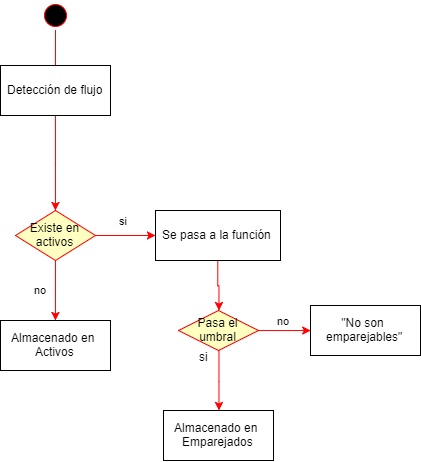
\includegraphics[width=0.9\textwidth]{imagenes/nacimiento.png}
  \centering
  \caption{Detección de un nuevo flujo.}\label{fig.nacimiento}
\end{figure}

\intro En la Figura \ref{fig.muerte}, se puede ver cómo se comportará el sistema cuando vaya a eliminar un flujo de la memoria.


\begin{figure}[H]
  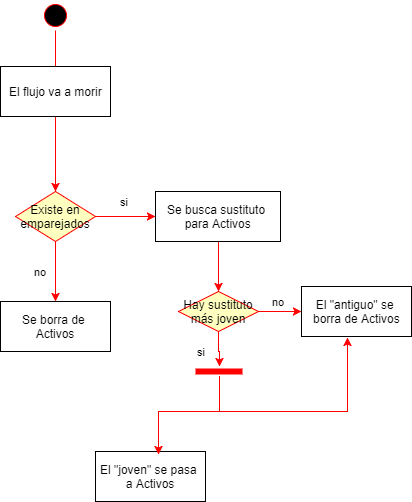
\includegraphics[width=0.9\textwidth]{imagenes/muerte.png}
  \centering
  \caption{Muerte de un flujo.}\label{fig.muerte}
\end{figure}

\intro Dependiendo del trato que se les vaya a dar a los flujos detectados se almacenarán en una lista o en otra. Estos pueden estar 
en diferentes estados, siendo estos los que se consideran:

\begin{itemize}
\item Activo. El flujo está activo y almacenado.
\item Emparejado. El flujo ha sido emparejado con otro flujo activo.
\item Finalizado. El flujo ha cumplido su tiempo de vida y es borrado de la memoria.
\end{itemize}

\intro Por lo tanto, cuando un flujo es detectado tendrá el estado activo. En función 
de los distintos flujos que se vayan detectando los flujos activos se irán comparando con los nuevos que se detecten, de modo que los 
nuevos que pasarán a estar emparejados. Si no se encuentra un flujo activo que coincida con sus parámetros los nuevos flujos serán 
almacenados como activos. Al último estado, finalizado, se podrá pasar tanto del estado activo, como del emparejado, con la diferencia 
de que de tratarse del primer caso deberá de ser borrado de la lista y se buscará un sustituto entre los emparejados con ese flujo. En 
el segundo caso no se borrará de la lista. La transición de estados se puede ver en la Figura \ref{fig.flujos}.

\begin{figure}[H]
  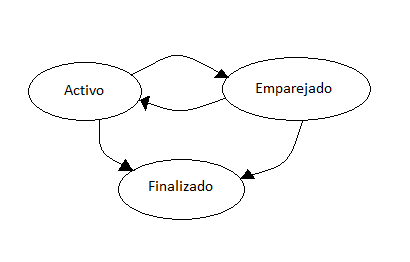
\includegraphics[width=0.7\textwidth]{imagenes/flujos.png}
  \centering
  \caption{Distintos estados de los flujos.}\label{fig.flujos}
\end{figure}

\intro Para el análisis será necesario disponer de tráfico. Este entrará en forma de traza, con formato \textit{pcap}. Las salidas 
se darán en forma de registros, en los cuales se mostrarán los flujos que han sido emparejados.

\intro La configuración de Bro, se realiza mediante la línea de comandos, cuando se va a lanzar el programa. Por lo tanto, para el 
módulo que se está describiendo es preciso únicamente activar la opción \textit{-r}, de forma que se le permita leer el archivo que se 
le pasará como parámetro a continuación. En el caso de que se quiera escanear el tráfico de una interfaz, se deberá de activar la 
opción \textit{-i} indicando a continuación el nombre de la interfaz a analizar. Se puede ampliar esta información leyendo la ayuda de 
Bro con \textit{-h}.

\section{Módulo y funciones}

Las funcionalidades que se espera que tenga este módulo en esencia son dos, la detección y almacenado 
del tráfico, y la aplicación de la fórmula para conocer si dos flujos son emparejables, a los distintos flujos que 
se han detectado. De una forma más amplia las funciones del módulo serán las siguientes. 

\begin{itemize}
\item \textit{Función que aplique la fórmula de emparejamiento}. 
\intro A esta función se le pasará dos flujos, de forma que se aplique la fórmula y devuelva un número, el cual 
será el que indique si los flujos son emparejables o no.
\item \textit{Funciones que detecten el tráfico}. 
\intro Esto se hará con los eventos de Bro. Los eventos detectarán el tipo de tráfico que se está analizando 
y aplicarán la función anterior.
\intro Tras el uso de esta fórmula se almacenará o no el flujo que está siendo analizado. Por lo tanto 
será necesario el uso de algún tipo de contenedor para este cometido.
\end{itemize}

\intro Lo que se espera es capturar el tráfico de la capa de transporte. Dicho tráfico se corresponde a los 
protocolos \textit{TCP y UDP}. Por lo tanto será necesario ver que tipo de eventos son los que controlan el tráfico 
de estos dos protocolos. A su vez, se tendrá que crear variables globales para el almacenamiento de los flujos que sean emparejables 
y los que estén activos.

\intro Las entradas y salidas son de fácil gestión. Las entradas de tráfico podrán ser mediante archivos o 
analizando directamente el tráfico de la red. Las salidas, por su parte, serán mediante registros. Esto puede 
suponer cierto inconveniente si se obtienen demasiadas salidas. También se pueden guardar las salidas en un 
fichero mediante el carácter \textit{mayor que} . Con esto se guardará en un fichero en la ruta que se especifique, siendo el 
posterior análisis mucho más cómodo desde, por ejemplo, un editor de texto.

\intro Se debe de tener en cuenta que siempre se podrá extender la funcionalidad del módulo. Pero de momento no 
resulta interesante. La posible extensión correspondería a posibles trabajos futuros.

\intro Para realizar este módulo es necesario conocer como gestiona los flujos Bro y de que forma se mantendrán 
los que son emparejados y los que están activos.

\section{Gestión de flujos}

La gestión de los flujos se realiza completamente mediante los eventos de Bro.

\intro Existen eventos que gestionan el nacimiento y la muerte de los flujos, siendo estos dos eventos genéricos. Por el contrario, 
se deberán de usar los distintos eventos especializados para gestionar los distintos tipos de tráfico.

\intro De esta forma, se tendrán eventos únicos que detectarán el tráfico \textit{TCP} y otros para \textit{UDP}. Una vez dentro, se 
realizarán los pasos necesarios para llevar el flujo detectado hasta la función de evaluación.

\intro En el evento correspondiente al nacimiento de un flujo, se deberá de analizar si se tiene otro con el que compararlo, o directamente se almacena con los demás flujos activos.

\intro En cuanto al evento relacionado con la muerte de un flujo, se tendrá que evaluar si en la lista de emparejados se tiene otro, al cual le quede más tiempo de vida, para que lo reemplace en la lista de flujos activos.

\intro A continuación se verán las estructuras de datos necesarias para llevar a cabo el desarrollo del módulo.

\section{Estructuras de datos}

Las principales estructuras de datos que se necesitan para el desarrollo de este trabajo serán dos tablas, \textit{table} 
\cite{brotable}, de vectores para el almacenamiento de los flujos activos y los emparejados. Los vectores son iguales que en cualquier 
otro lenguaje de programación, mientras que las tablas son parecidas a los \textit{maps} de \textit{C++}. Aunque esto se explicará más 
detalladamente en el capítulo \ref{implementacion}.

\intro Dichas estructuras de almacenamiento, deberán de ser capaces de estar ordenadas por las IP's y los puertos. Esto se obtiene 
haciendo que las tablas estén compuestas de vectores, por lo cual, se obtendrá una matriz bidimensional indexada. Por lo tanto se 
consigue que el acceso a los datos sea mucho más rápido. Incluso se podría prescindir de bucles, los cuales pueden acabar 
siendo un problema en cuanto a rendimiento si se analiza mucho tráfico.

\intro Bro proporciona cierto tipos de datos muy interesantes, los cuales además, incluyen mucha más información. Algunos de estos 
tipos de datos son. 

\begin{itemize}

\item \textit{connection}. 

\intro Este tipo de dato es el flujo en sí. Por lo tanto será de vital importancia comprenderlo para poder trabajar como se desea.

\intro Dentro de \textit{connection} existe un registro llamado \textit{id}, el cual esta compuesto por el tipo de dato \textit{conn\_id} \cite{broconnid}. Este dato sirve para identificar los flujos mediante una tupla formada por 4 datos. Estos datos son los que se 
precisan para indexar la matriz bidimensional.

  \begin{itemize}

  \item \textit{addr}. Este tipo de dato representa una IP. Reconoce tanto IPv4 como IPv6. Este tipo de dato puede 
  ser comparado e incluso ordenado mediante operadores \cite{broaddr}.

  \item \textit{port}. Este tipo es el usado para los puertos. Además del número, también indica el 
  protocolo de la capa de transporte que usa. Soporta la comparación y ordenación, pero no por el número, sino por 
  el tipo de protocolo \cite{broport}.
  \end{itemize}
  
\intro Se puede consultar más información sobre el tipo de dato \textit{connection} en \cite{connectiontype}.

\item \textit{time}. 

\intro Aunque en otros lenguajes se pueden crear estructuras que se asemejen a este tipo, Bro da un tipo de dato muy completo. Además, 
se puede operar sobre él desde el principio, siendo una gran ventaja a la hora de calcular el tiempo de inicio de los flujos. Más 
información en \cite{timetype}.

\intro Es importante entender que para realizar el cálculo para el emparejamiento de flujos, se necesita el 
\textit{timestamp} del primer paquete de cada flujo, pues será sobre este tiempo sobre el que se apoye el 
cálculo del emparejamiento.

\end{itemize}

\intro Estos dos tipos de datos a parte de ser los más interesantes para el cálculo del emparejamiento, también 
serán los más utilizados junto a los contenedores para los flujos. Existen más tipos de datos e incluso los hay que 
extienden la información disponible sobre los flujos. Más información sobre distintos tipos de datos en \cite{conntype}.

%
\chapter{Implementación}

Ahora vamos a proceder a explicar cómo se ha solucionado los problemas 
propuestos, siendo estos explicados a través del programa que se ha 
realizado, quedando así más clara la explicación.
\intro
\begin{lstlisting}[style=CodigoC]
## funcion para la comparacion de los flujos, c1 el flujo que esta en el set conex y c2 para el flujo que es candidato a guardarse en empa
function emparejamiento(c1: connection, c2: connection ):double {

  local Nip=1; ## Variable para saber cuantas conexiones tenemos
  local Po1: count; ## Puerto origen del primer flujo
  local Po2: count; ## Puerto origen del segundo flujo
  local Pd1: count; ## Puerto destino del primer flujo
  local Pd2: count; ## Puerto destino del segundo flujo
  local k1 = 1;  ## Variable fija
  local k2 = 10; ## Variable fija
  local dt: double; ## Variable para la diferencia de los tiempos
  local resultado = 0.0; ## Lo ponemos a 0
  print c1$uid;
  print c2$uid;
## Podemos saltarnos este bucle si inicializamos Nip a 1
  ## for (s in conex){

  ##   if((s$id$orig_h == c1$id$orig_h) && (s$id$resp_h == c1$id$resp_h) && (s$id$orig_p == c1$id$orig_p) && (s$id$resp_p == c1$id$resp_p)){
  ##           Nip=Nip+1;
  ##           print fmt("Numero de Nip sin table: %d", Nip);
  ##           break;
  ##   }
  ## }

  if(c1$uid==c2$uid){
    print fmt("Son el mismo flujo, no se realiza incremento en Nip");
  }else{
## Este bucle lo puedo hacer sin ningun problema, pues en los eventos todavia no se ha dicho que se guarde en el set
  for (i in empa){
    if((i$id$orig_h == c2$id$orig_h) && (i$id$resp_h == c2$id$resp_h) && (i$id$orig_p == c2$id$orig_p) && (i$id$resp_p == c2$id$resp_p)){
            Nip=Nip+1;

    }
  }
  print fmt("Numero de Nip en table: %d", Nip);
  informacion_coincidencia(c1,c2);
  print fmt("Tiempo de inicio del flujo: %s", |c1$start_time|);
  print fmt("Tiempo de inicio del flujo: %s", |c2$start_time|);
  ## Para dp1 y dp2 que son 1-norm usamos la "Manhattan norm" que dice lo siguiente: SAD(x1,x2) = sumatoria(x1i - x2i)
  ## k1 y k2 son dos variables que nosotros le ponemos de forma manual, en este caso las pondremos como locales con 1 y 10 respectivamente
  ## dt es la diferencia de tiempo entre los time stamp de los primeros flujos de los flujos
  ## el tipo time se supone que es como un double, por lo tanto podremos restarlos sin problemas
  ## para la comparacion de puertos primero tendremos que hacer uso de la funcion  port_to_count [https://www.bro.org/sphinx/scripts/base/bif/bro.bif.bro.html#id-port_to_count]
  ## la cual nos pasa el puerto, que recordamos que va tambien con un string en el cual se nos dice que tipo es, a un
  ## valor numerico que si podremos restar sin problemas
  ## La funcion quedaria asi: (Nip-1)+(1/(dp1+k1))+(1/(dp2+k1))+(1/(dt+k2))
  Po1=port_to_count(c1$id$orig_p);
  Pd1=port_to_count(c1$id$resp_p);
  Po2=port_to_count(c2$id$orig_p);
  Pd2=port_to_count(c2$id$resp_p);
  ## local t1: double;
  ## local t2: double;
  ## t1 = time_to_double(c1$start_time);
  ## t2 = time_to_double(c2$start_time);

  dt=(|c1$start_time| - |c2$start_time|);

  ## print fmt("Tiempo paquete 1: %s", t1);
  ## print fmt("Tiempo paquete 2: %s", t2);
  print fmt("Diferencia de tiempo: %s", dt);
  resultado=(Nip-1)+(1/((Po1-Po2)+k1))+(1/((Pd1-Pd2)+k1))+(1/(dt+k2));
 }
 return resultado;

}
\end{lstlisting}
En este trozo de código se muestra la función que se usa para devolver 
el resultado de la función de comparación. El resultado será comparado 
con el umbral que nosotros definimos, haciendo que si dicho resultado 
es mayor que el umbral serán emparejables y por tanto serán guardados 
en un table[connection] of connection, lo que sería comparable en C++ 
con un map. Decidimos guardarlos dentro de cada uno de los eventos que 
lanzamos cuando Bro reconoce un determinado protocolo, dichos eventos son:
\intro
\begin{itemize}
\item connection\_established, el cual se lanza cuando Bro localiza un SYN-ACK que corresponda a un handshake de TCP.
\item connection\_finished, el cual lanza Bro cuando una conexión TCP finaliza de forma normal. 
\item udp\_request, el cual se lanza cuando Bro localiza un flujo que corresponde con UDP lanzado desde el origen.
\item udp\_reply, que es lanzado por Bro cuando localiza una respuesta a un flujo del anterior evento.
\item icmp\_echo\_request, lanzado por Bro cuando localiza un flujo de tipo ICMP de echo.
\item icmp\_echo\_reply, el cual es lanzado por Bro cuando localiza una respuesta a los flujos del evento anterior.
\end{itemize}

Dentro de estos eventos descritos se realiza la comprobación de que dos 
flujos se pueden comparar, ya que tienen los mismos IP’s y puertos de 
origen y destino. Una vez en la función de comparación se almacenarán 
dichos puertos, pasándolos al tipo count para su uso en la función, se 
establecerán dos constantes, se calculará la diferencia de tiempo y en 
una variable se almacenará el número de flujos que hay con esos datos. 
Cuando realicemos esto, aplicaremos la función de cálculo y podremos 
decir si los flujos son emparejables.
\intro
Para mostrar la información de los flujos tenemos dos opciones, de las 
cuales mostramos el código a continuación:
\intro
\begin{lstlisting}[style=CodigoC]
## Creo funcion auxiliar para ver la informacion del flujo nuevo que se añade, no de todos los flujos todo el rato
function informacion_flujo(c: connection){
    print fmt("Informacion del flujo nuevo IPo: %s , Po: %s , IPd: %s , Pd: %s ", c$id$orig_h, c$id$orig_p, c$id$resp_h, c$id$resp_p);
}


## Creo funcion auxiliar para ver la informacion del flujo que se coincide
function informacion_coincidencia(c: connection, p: connection){
    print fmt("Informacion del primer flujo  IPo: %s , Po: %s , IPd: %s , Pd: %s ", c$id$orig_h, c$id$orig_p, c$id$resp_h, c$id$resp_p);
    print fmt("Informacion del flujo coincidente  IPo: %s , Po: %s , IPd: %s , Pd: %s ", p$id$orig_h, p$id$orig_p, p$id$resp_h, p$id$resp_p);
}

La función informacion_flujo sirve para mostrar la información del flujo relativa a las IP’s y a los puertos que contiene. Por su parte la función informacion_coincidencia sirve para mostrar la información de dos flujos a la vez, mostrando sus IP’s y sus puertos, la cual será usada para mostrar al final la información que tenemos en la tabla y el flujo con el que coincide en el set de comparaciones.

En el programa se hace uso también de un evento para eliminar los flujos que estén a punto de morir, este evento es:

connection_state_removed, evento que lanza Bro cuando va a eliminar de la memoria un flujo activo.

## Cuando la conexion va a ser borrada la eliminamos del set y en caso de tener otra conexion en el empa la añadimos
## se obtienen los mismos flujos añadidos que eliminados, por lo tanto hay que controlar cuando lo añadimos y cuando lo eliminamos
## Sirve para TCP, UDP e ICMP
## Generated when a connection’s internal state is about to be removed from memory. Bro generates this event reliably
## once for every connection when it is about to delete the internal state. As such, the event is well-suited for
## script-level cleanup that needs to be performed for every connection.
## This event is generated not only for TCP sessions but also for UDP and ICMP flows.
event connection_state_remove(c: connection){

## Creo un connection local para poder pasarlo de empa a conex
   local cl: connection;
## Variable booleana para controlar el acceso al set
   local esta = F;

## for que va recorriendo el set y haciendo comparaciones
    for(s in empa){
      if((s$id$orig_h == c$id$orig_h) && (s$id$resp_h == c$id$resp_h) && (s$id$orig_p == c$id$orig_p) && (s$id$resp_p == c$id$resp_p)){
## Si se dan todas las condiciones la variable booleana de control de acceso al set se cambia a true, T
              esta=T;
## Al existir otro flujo lo copiamos en cl
              cl=s;
              break;
      }
    }

    ## Aqui si tenemos otro flujo igual al que vamos a eliminar lo metemos en conex para que ocupe el lugar del que vamos a borrar
    ## Con la variable booleana controlamos el decrecimiento del set
    if (esta==T){
      delete conex[c];
      add conex[cl];
      delete empa[cl];
      ## print fmt("Hemos borrado");
      ## print empa[cl];
    } else {
      delete conex[c];
    }
    elimi=elimi+1;
    ## Quitamos uno al tamaño del set
    tams=tams-1;
    esta=F;
    ##  print fmt("Tamanio del set: %d", tams);
    ##  informacion_flujo(c);

}
\end{lstlisting}

En nuestro caso antes de eliminarlo del set de comparaciones 
lo que hacemos es ver si en la tabla de emparejados existe un 
flujo con los mismos datos, en caso de que exista borramos el 
flujo del set, pasamos al set el flujo de la tabla de emparejados 
y este flujo lo eliminamos de la tabla. La ventaja que tiene 
esto es que el timestamp será actualizado, haciendo que la 
diferencia de los tiempos de dos flujos no sea demasiado grande 
y por lo tanto teniendo más posibilidades de que exista algún 
flujo que sea emparejable con el nuevo. En caso de que no exista 
un flujo con las características deseadas para la sustitución en 
el set de conexiones, simplemente será borrado, si no ha tenido 
ningún flujo con el cual ha sido emparejado en todo el uso del 
programa, este flujo borrado nunca será mostrado, en caso de que 
si lo tuviese, el flujo siempre estará almacenado en una tabla 
que mostramos al finalizar el programa.
\intro
Para añadir flujos al set de conexiones, tenemos un evento 
dedicado a ello:
\intro
\begin{itemize}
\item new\_connection, Bro lanza este evento cada vez que detecta un flujo que era desconocido.
\end{itemize}

\begin{lstlisting}[style=CodigoC]
## Cada vez que entra un nuevo flujo lo comparo con lo que ya tengo en el set
## Este evento se lanza con cada nueva conexion de un flujo que no sea conocido
## Generated for every new connection. This event is raised with the first packet of a previously unknown connection. Bro uses a flow-based definition of “connection” here that includes not only TCP sessions but also UDP and ICMP flows.
event new_connection(c: connection){

## Si el set esta vacio meto el primer flujo
   if(tams==0){
    add conex[c];
   }
## Sumamos uno al tamaño del set
    tam=tam+1;

## Variable booleana para controlar el acceso al set
     local met = F;

## for que va recorriendo el set y haciendo comparaciones
     for(s in conex){
## Copiamos en la variable local para comparar con todo lo que hay en el set
       if((s$id$orig_h != c$id$orig_h) && (s$id$resp_h != c$id$resp_h) && (s$id$orig_p != c$id$orig_p) && (s$id$resp_p != c$id$resp_p)){
               ## Si se dan todas las condiciones la variable booleana de control de acceso al set se cambia a true, T
               met=T;
       }

     }
    ## Con la variable booleana controlamos el crecimiento del set
     if (met==T){
       add conex[c];
       tams=tams+1;
       ## print fmt("Meto un flujo nuevo por la conexion de origen distinta");
     }
     met=F;
    ## print fmt("Numero de flujos al momento: %d", tam);
    ## print fmt("Tamanio del set: %d", tams);
    ## informacion_flujo(c);

}
\end{lstlisting}

Lo primero que debemos de hacer es ver si el tamaño del set de 
conexiones es 0, en caso de serlo añadimos el flujo directamente, 
en caso de que no sea 0 tenemos que ver primero si tenemos un flujo 
con los datos de comparación iguales, en caso de tenerlo el flujo 
no será añadido, en caso de que no exista otro flujo con los mismos 
datos de comparación lo guardaremos.
\intro
Por último usamos dos eventos en el programa para ver cuando se 
lanza y cuando finaliza el programa:
\intro
\begin{itemize}
\item bro\_init, evento que se lanza cuando iniciamos Bro.
\item bro\_done, evento que se lanza cuando Bro va a terminar.
\end{itemize}
\intro
\begin{lstlisting}[style=CodigoC]
## Evento que se lanza cuando se inicia BRO.
event bro_init(){

  print fmt("Hora de inicio: %s", current_time());

}

## Evento que se genera cuando BRO va a tenerminar, menos si se realiza mediante una llamada a la funcion exit (ver documentacion)
event bro_done(){

  ## Mostramos lo que tenemos en la tabla de emparejados
  for(s in emparejados){
    ## print fmt("Tamaño de la fila de la tabla: %d", |empa[s]|);
    ## print fmt("Tenemos: %s en %s a %s en %s", emparejados[s]$id$orig_h, emparejados[s]$id$orig_p, emparejados[s]$id$resp_h, emparejados[s]$id$resp_p);
    ## print fmt(" de %s en %s a %s en %s", s$id$orig_h, s$id$orig_p, s$id$resp_h, s$id$resp_p);
    informacion_coincidencia(emparejados[s], s);
  }

  ## for(i in emparejados){
    ## print fmt("Tenemos lo siguiente:");
    ## print emparejados[i];
  ## }

  print fmt("Total de flujos: %d", tam);
  print fmt("Hora de finalizacion: %s", current_time());
}
\end{lstlisting}

En el primer evento solamente mostramos la hora a la que se 
inicia el programa mediante la función current_time. En el 
evento del final mostramos los flujos que han sido emparejados 
y mostramos la hora de finalización del programa.

%
\chapter{Evaluación y pruebas}\label{evaluacion}

En este capítulo se realizarán las pruebas al sistema. Para ello, a partir de un archivo que contenga una traza de tráfico, se 
analizará con el módulo creado, de forma que se compruebe que se crea el registro correspondiente y que este contiene los flujos 
emparejados.

\intro Se añadirán capturas de pantalla en las que se vea claramente que todo funciona como debería, así mismo, se podrán comprobar 
los registros que se creen en el repositorio de GitHub \citep{repo}.

\section{Establecer las variables}

Lo primero que se hará, será establecer las variables \textit{k1} y \textit{k2}. Estas se definen de forma global al principio 
del módulo. Cómo ya se vio anteriormente, en la explicación de la ecuación \ref{ecug}, sus valores estarán comprendidos entre 0,1 y 
10000. Como se puede ver, en la Figura \ref{fig.variables}, para las pruebas se han establecido los valores en 1 y 100.

\begin{figure}[H]
  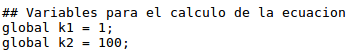
\includegraphics[width=0.6\textwidth]{imagenes/variables.png}
  \centering
  \caption{Valores de las variables \textit{k1 y k2}.}\label{fig.variables}
\end{figure}

\intro A su vez, también será necesario definir el umbral que servirá para descartar o aceptar emparejamientos. Como se puede ver en 
la Figura \ref{fig.definirumbral}, en el caso de estas pruebas el valor será de 1.

\begin{figure}[H]
  
\includegraphics[width=0.3\textwidth]{imagenes/definirumbral.png}
  \centering
  \caption{Valor de la variable \textit{umbral}.}\label{fig.definirumbral}
\end{figure}


\section{Prueba del módulo}

A continuación, se realizará una prueba del módulo, con las variables anteriormente descritas, para comprobar que todo funciona 
correctamente.

\intro Como se puede ver en la Figura \ref{fig.terminal}, para lanzar el módulo, será necesario indicar el archivo que se va a 
analizar.

\begin{figure}[H]
  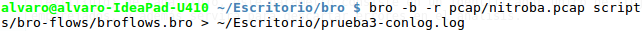
\includegraphics[width=1\textwidth]{imagenes/terminal.png}
  \centering
  \caption{Lanzamiento del módulo para realizar el análisis.}\label{fig.terminal}
\end{figure}

\intro Cabe destacar, que para la depuración se muestran mensajes por terminal. Estos son escritos en un archivo mediante el carácter \textit{mayor que}, de forma que se pueda realizar búsquedas sobre ellos. En la Figura \ref{fig.salida} se puede ver una muestra de estos mensajes,en los cuales se muestra el \textit{uid} de los dos flujos, el número de IP's coincidentes y los puertos de ambos flujos.

\begin{figure}[H]
  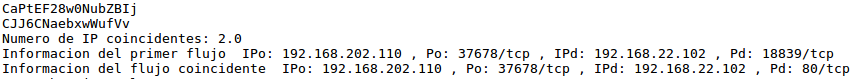
\includegraphics[width=1\textwidth]{imagenes/salida.png}
  \centering
  \caption{Muestra de los mensajes de depuración.}\label{fig.salida}
\end{figure}

\intro En el registro que se crea cada vez que se ejecuta el análisis, además de las IP's y los puertos, también se muestran los 
\textit{uid} de cada flujo, este parámetro consiste en un identificador único de flujo. Esto ayudará a identificar los flujos que son 
emparejados y además, servirá para descartar errores en el análisis.

\intro En la Figura \ref{fig.lognitroba}, se puede comprobar el registro que se genera al analizar un archivo. En este caso, el 
archivo analizado ha sido \textit{nitroba.pcap}, cuyo peso es de 56,2 MB, el cual se encuentra accesible desde la web de Bro. Esta 
traza se corresponde con un escenario de prueba realizado por una universidad sudafricana. 

\begin{figure}[H]
  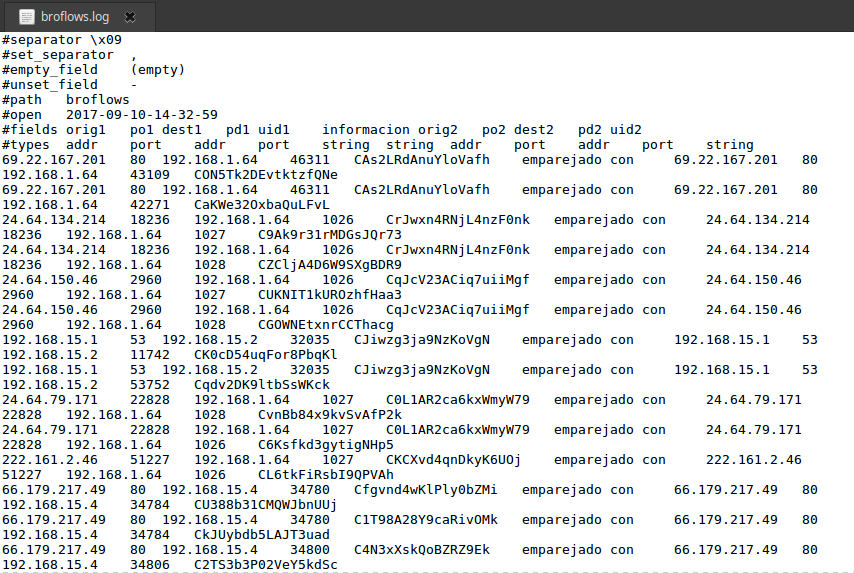
\includegraphics[width=0.9\textwidth]{imagenes/lognitroba.png}
  \centering
  \caption{Log del archivo \textit{nitroba.pcap}.}\label{fig.lognitroba}
\end{figure}

\intro En el registro se pueden ver los flujos emparejados. Al trabajar con una traza pequeña, cabe esperar que sean pocos los 
resultados, en cuanto a número de flujos emparejados. Este tipo de archivos son ideales para realizar las pruebas, pues tarda muy poco 
el sistema en analizarlos, siendo en este caso 1 segundo el tiempo utilizado.

\intro En la Figura \ref{fig.dosflujosemparejados}, se encuentran dos emparejamientos que pertenecen a la misma clase. Esto se puede 
comprobar, ya que el primer flujo tiene el mismo \textit{uid} y los flujos con los que se empareja no.

\begin{figure}[H]
  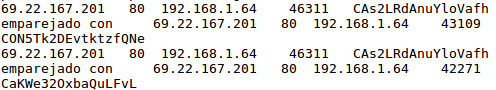
\includegraphics[width=1\textwidth]{imagenes/dosflujosemparejados.png}
  \centering
  \caption{Dos flujos emparejados.}\label{fig.dosflujosemparejados}
\end{figure}

\intro Por lo tanto, con esto se puede afirmar que el módulo empareja de forma adecuada los flujos.

\intro En cuanto al borrado de flujos, en la Figura \ref{fig.borrado}, se puede ver que el \textit{uid} de un flujo activo solo existe 
dos veces, siendo borrado de memoria después de esas comparaciones. Por lo tanto, se puede afirmar que el módulo borra de forma 
adecuada los flujos cuando ya no los necesita.

\begin{figure}[H]
  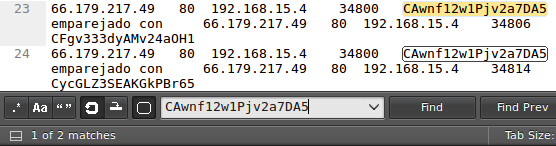
\includegraphics[width=1\textwidth]{imagenes/borrado.png}
  \centering
  \caption{Borrado de flujos.}\label{fig.borrado}
\end{figure}

\intro Además, la única información accesible es la que está en el registro, por lo que no se entra dentro de los paquetes y se 
garantiza la privacidad.

\section{Escenarios reales}

Una vez que se ha comprobado que todo funciona de forma correcta con un archivo pequeño, se pasará a analizar un archivo más grande, 
correspondiente a un escenario real. En este caso se trata de \textit{maccdc2012\_00004.pcap}, correspondiente al \textit{National 
CyberWatch Mid-Atlantic Collegiate Cyber Defense Competition} o \textit{MACCDC} \cite{maccdc}. En este archivo se encuentra el tráfico 
de un día y ocupa cerca de 1.1 GB.

\intro En la Figura \ref{fig.logmaccdc}, se puede ver que al realizar el análisis con el módulo, se obtiene un registro mucho más 
extenso. De hecho, tarda cerca de 50 minutos en realizarlo, frente al segundo que tardaba el análisis del archivo anterior.

\begin{figure}[H]
  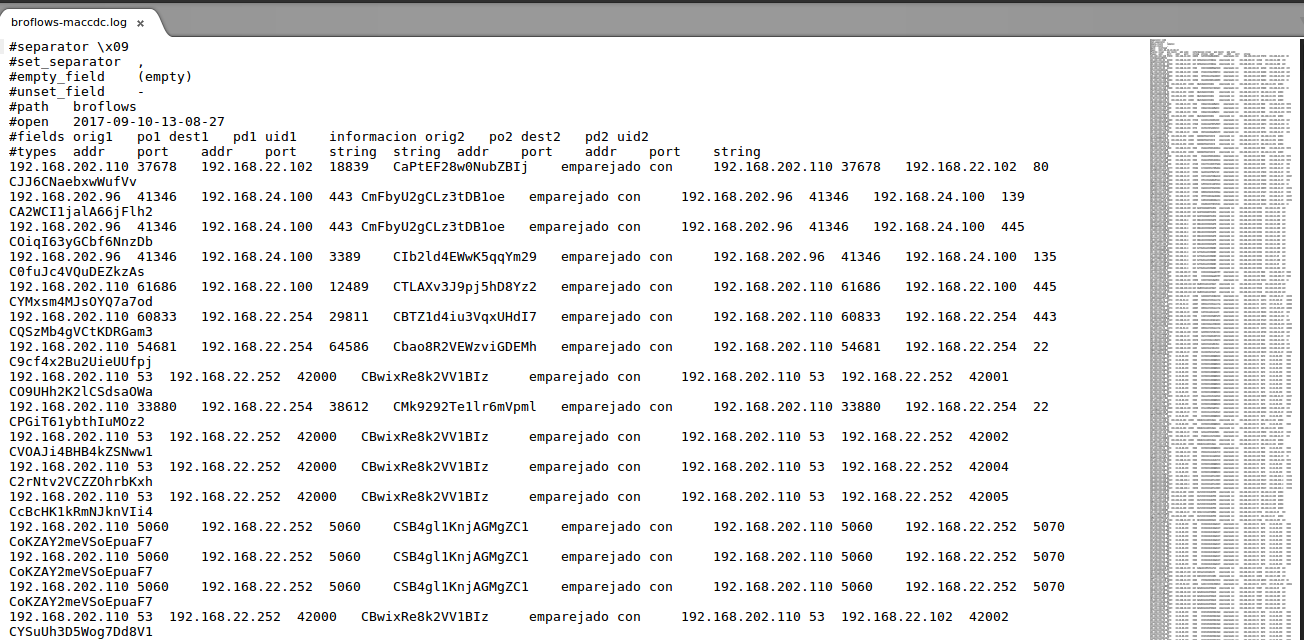
\includegraphics[width=1\textwidth]{imagenes/logmaccdc.png}
  \centering
  \caption{Log del archivo \textit{maccdc2012\_00004.pcap}.}\label{fig.logmaccdc}
\end{figure}

\intro Mientras que en el análisis anterior se llegaba como mucho a emparejar tres flujos, en este se pueden llegar a obtener unos 8 
flujos emparejados, como se ve en la Figura \ref{fig.flujosemparejados}. Cabe destacar, que estos resultados variarán en función de los valores que se le asignen a los parámetros y al umbral.

\begin{figure}[H]
  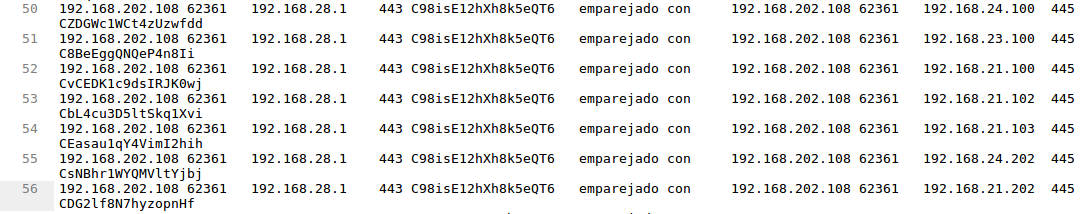
\includegraphics[width=1\textwidth]{imagenes/flujosemparejados.png}
  \centering
  \caption{Flujos emparejados.}\label{fig.flujosemparejados}
\end{figure}

\intro Y de nuevo, si se realiza una búsqueda usando el \textit{uid} del primer flujo, se verá que no se muestra más veces, por lo que 
se realiza el borrado de la tabla de activos correctamente.

\intro Por lo tanto, vemos que también es escalable siendo analizado en este apartado un archivo de 1.1 GB, y en el anterior un 
archivo de 0.05 GB. Obviamente, el tiempo no se mantiene estable, pues es imposible analizar tanta información en un segundo. Pero, este archivo contiene el tráfico de todo un día, por lo que un análisis de esa cantidad de tráfico en menos de 50 minutos, es algo 
aceptable.

%
\chapter{Conclusiones y trabajo futuro}\label{conclusiones}

En este capítulo se expondrán las conclusiones alcanzadas después de realizar todo el trabajo, así como el posible trabajo futuro.

\section{Conclusiones}

Tras todo lo expuesto a lo largo de esta memoria, y tras ver los resultados en el capítulo \ref{evaluacion}, se llega a la conclusión 
de que la técnica propuesta por los investigadores del departamento de Teoría de la Señal, Telemática y Comunicaciones de la 
Universidad de Granada, es una técnica completamente funcional. Además, mejora los dos aspectos que fallan en la Inspección Profunda 
de Paquetes.

\begin{itemize}
\item \textit{Privacidad}. Este aspecto se respeta, pues los únicos datos analizados y mostrados en el registro generado, son las 
IP's, los puertos y los \textit{uids}, siendo además usado el tiempo de inicio del primer paquete del flujo. Por lo tanto, no se entra 
dentro del \textit{payload} de los paquetes, lo cual puede ser ilegal en algunos países.

\item \textit{Escalabilidad}. Se ha podido comprobar que un archivo de 1.1 GB, correspondiente al tráfico de un día entero, es 
analizado en menos de una hora siendo un tiempo aceptable, teniendo presente la cantidad de flujos que existen dentro de ese fichero. 
Un archivo más pequeño y destinado a hacer pruebas, de 56.2 MB, es analizado en un segundo.
\end{itemize}

\intro Además, los datos volcados en el registro generado son útiles y sobre ellos se puede realizar una búsqueda rápida, de modo que 
se detectaría, por ejemplo, un ataque de denegación de servicio rápidamente, pudiendo el administrador del sistema realizar las 
acciones que crea convenientes.

\section{Trabajo futuro}

Se podría continuar trabajando sobre este módulo, de forma que se haga más rápido o detecte más tipo de tráfico. Algunas de las posibles mejoras son:

\begin{itemize}
\item Añadir otras funciones, de modo que se analice el tráfico a otros niveles, como podría ser a nivel de capa de aplicación. Esto podría realizarse mediante la incorporación de eventos que detecten actividad \textit{HTTP}, por ejemplo.
\item Extender las funcionalidades ya expuestas añadiendo, por ejemplo, nuevos eventos que detecten tráfico de tipo \textit{TCP}, ya 
que este módulo solamente tiene dos funciones que detectan este tipo de tráfico, siendo el inicio y el final del protocolo lo que es 
detectado.
\item Optimizar el almacenado de flujos. Se podría optimizar el módulo mejorando la forma en que son guardados los flujos, así 
como el borrado de los mismos.
\end{itemize}
%
%\input{capitulos/07_Pruebas}
%
%\input{capitulos/08_Conclusiones}
%
%%\chapter{Conclusiones y Trabajos Futuros}
%
%
\appendix
\newpage
\chapter{Instalación de Bro}

En este apartado se van a detallar los pasos para instalar Bro en un sistema Linux. 

\section{Descargar Bro}

Los binarios de Bro se pueden descargar desde la propia web de Bro \cite{brodownload}, o desde su repositorio de GitHub.

\intro A continuación, se recomienda seguir los pasos que nos detallan en su web \cite{broinstall}, aunque serán detallados aquí.

\intro Lo primero será decidir de donde descargar los binarios, se recomienda hacerlo desde el repositorio de GitHub, pues así será mucho más sencillo tenerlo actualizado. Para ello, se realizarán los siguientes pasos:

\begin{lstlisting}[style=Consola]
sudo apt-get install cmake make gcc g++ flex bison libpcap-dev libssl-dev python-dev swig zlib1g-dev
\end{lstlisting}

\intro De esta forma, se obtendrán los paquetes necesarios para que Bro funcione correctamente. A continuación, clonaremos el repositorio de GitHub de Bro, de la siguiente forma:

\begin{lstlisting}[style=Consola]
git clone --recursive git://git.bro.org/bro
\end{lstlisting}

\section{Instalación}

Para el proceso de instalación, será necesario, antes de ejecutar los comandos siguientes, estar en la carpeta \textit{bro} que se ha generado con la descarga. Una vez que se esté en dicha carpeta, se procederá a la instalación con los siguientes comandos:

\begin{lstlisting}[style=Consola]
./configure
make
make install
\end{lstlisting}

\intro Una vez realizados estos pasos, se tendrá Bro instalado y listo para usarse.
\newpage
\chapter{Uso del módulo creado}\label{cap.uso}

En este apartado se encontrará una pequeña guía de los comandos de Bro, así como una pequeña guía del uso del módulo creado.

\section{Comandos de Bro}

A continuación, se encontrará una lista de los comandos más interesantes de Bro.

\begin{lstlisting}[style=Consola]
    -b|--bare-mode                 | no carga los scripts del directorio base/
    -d|--debug-policy              | activa el modo debug
    -f|--filter <filter>           | filtro tcpdump
    -h|--help|-?                   | ayuda
    -i|--iface <interface>         | lee de la interfaz dada
    -r|--readfile <readfile>       | lee el archivo dado
    -s|--rulefile <rulefile>       | lee las reglas del archivo dado
    -t|--tracefile <tracefile>     | activa la ejecucion de trazas 
    -w|--writefile <writefile>     | escribe en el archivo dado
    -x|--print-state <file.bst>    | muestra el contenido del archivo de estado
    -C|--no-checksums              | ignaora checksums
    -F|--force-dns                 | fuerza DNS
    -N|--print-plugins             | muestra los plugins disponibles y sale
    -Q|--time                      | muestra el tiempo de ejecucion en stderr
    -R|--replay <events.bst>       | repite los eventos
    -X|--broxygen <cfgfile>        | genera la documentacion basada en el archivo de configuracion dado   

\end{lstlisting}

\section{Uso de Bro}

Para usar Bro se tendrá que hacer lo siguiente.

\begin{lstlisting}[style=Consola]
	bro [opciones] [archivos]
\end{lstlisting}

\intro Pero antes de la ejecución de Bro, se tendrá que fijar el \textit{PATH} en la carpeta de Bro.

\begin{lstlisting}[style=Consola]
	export PATH =/usr/local/bro/bin:$PATH
\end{lstlisting}

\intro Una vez realizado este paso, se podrá ejecutar el módulo creado, de la siguiente forma.

\begin{lstlisting}[style=Consola]
	bro -b -r pcap/nitroba.pcap scripts/bro-flows/broflows.bro
\end{lstlisting}


\nocite{*}
\bibliographystyle{unsrtnat}
\bibliography{bibliografia/bibliografia}
\addcontentsline{toc}{chapter}{Bibliografía}

%
%\appendix
%\input{apendices/manual_usuario/manual_usuario}
%%\input{apendices/paper/paper}
%\input{glosario/entradas_glosario}
% \addcontentsline{toc}{chapter}{Glosario}
% \printglossary
\chapter*{}
\thispagestyle{empty}

\end{document}
